\subsection{MetaClust}
By clicking toolsets and then metaClust,
users are directed to metaClust home page as Figure~\ref{fig:metaClustHome}.

\begin{figure}[H]
\begin{center}
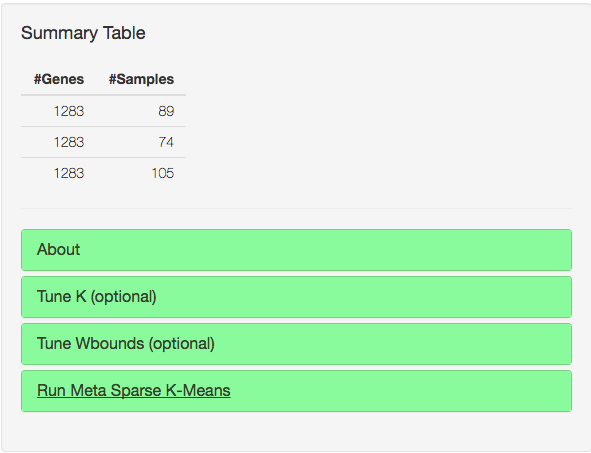
\includegraphics[scale=0.35]{./figure/metaClust/metaClustHome}
\caption{GUI Preprocessing page}
\label{fig:metaClustHome}
\end{center}
\end{figure}
On the top left panel users can see data summary Table.
Below there are 4 tabs.
\subsubsection{About}
About tab includes basic introduction of metaClust.
Starting with multiple studies, 
we could run MetaSparseKmeans with pre-specified number of clusters (K) and gene selection tuning parameter (Wbounds).
If you are not sure about what are good K and Wbounds, please try Tune K and Tune Wbounds panel.

\subsubsection{Tune K}
If the users are not sure what is number of clusters,
they can start to use the Tune K panel as in Figure~\ref{fig:metaClusttuneK}.
\begin{figure}[H]
\begin{center}
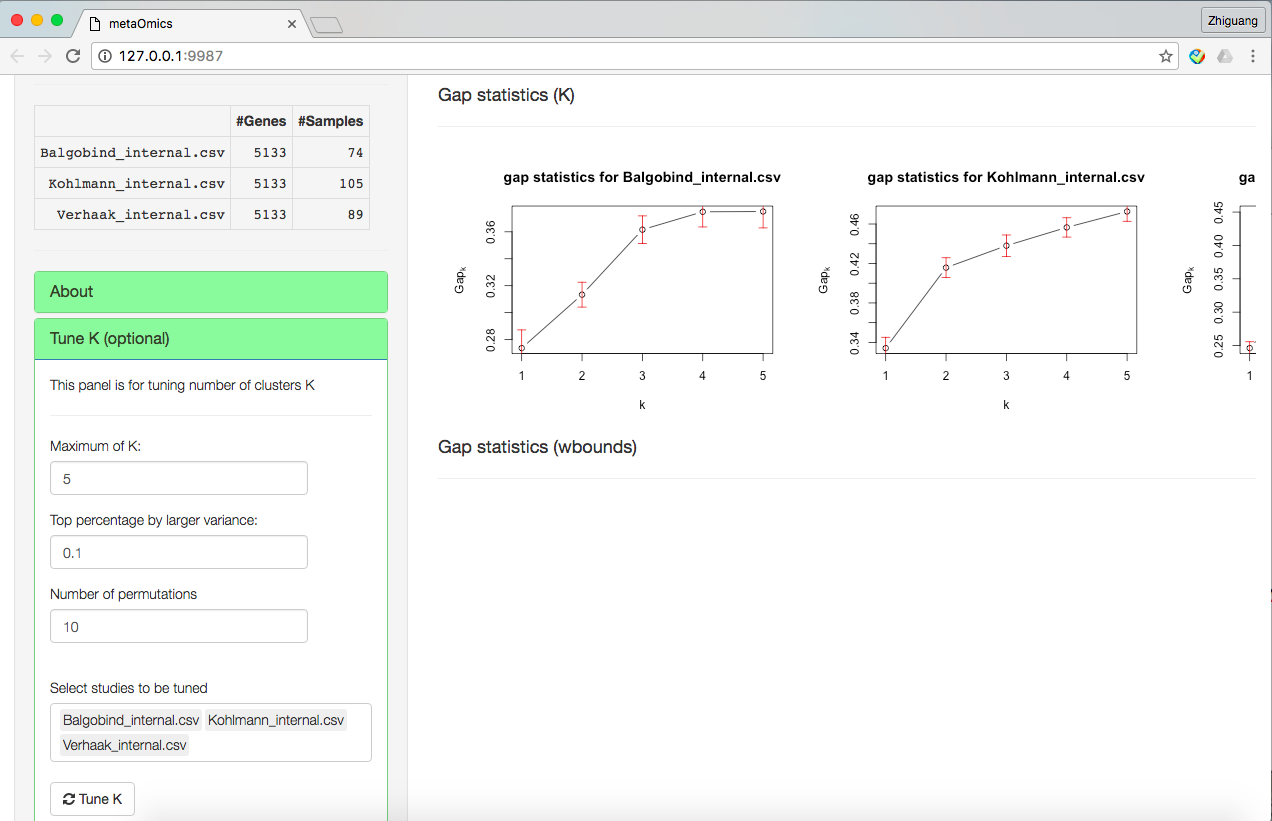
\includegraphics[scale=0.35]{./figure/metaClust/tuneK}
\caption{GUI Preprocessing page}
\label{fig:metaClusttuneK}
\end{center}
\end{figure}
Users will use gap statistics to get optimal K for each individual study.
Users need to specify maximum number of K, which the algorithm will search number of studies from 1 to K.
Top percentage p\% by larger variance means that we will use top p\% larger variance genes to perform gap statistics.
Number of permutation is number of bootstrap samples for gap statistics.
After selecting studies to be tuned and clicking button ``Tune K",
we will obtain gap statistics plat as in Figure~\ref{fig:metaClusttuneK}.
A good K is selected such that the $\mbox{Gap}_k$ is maximized or stablized.
From the figure, K=3 is prefered.


\subsubsection{Tune Wbounds}
Wbounds directly control number of features selected by metaClust.
If the users are not sure what is a good Wbound,
they can start to use the Tune Wbounds panel as in Figure~\ref{fig:metaClusttuneW}.
\begin{figure}[H]
\begin{center}
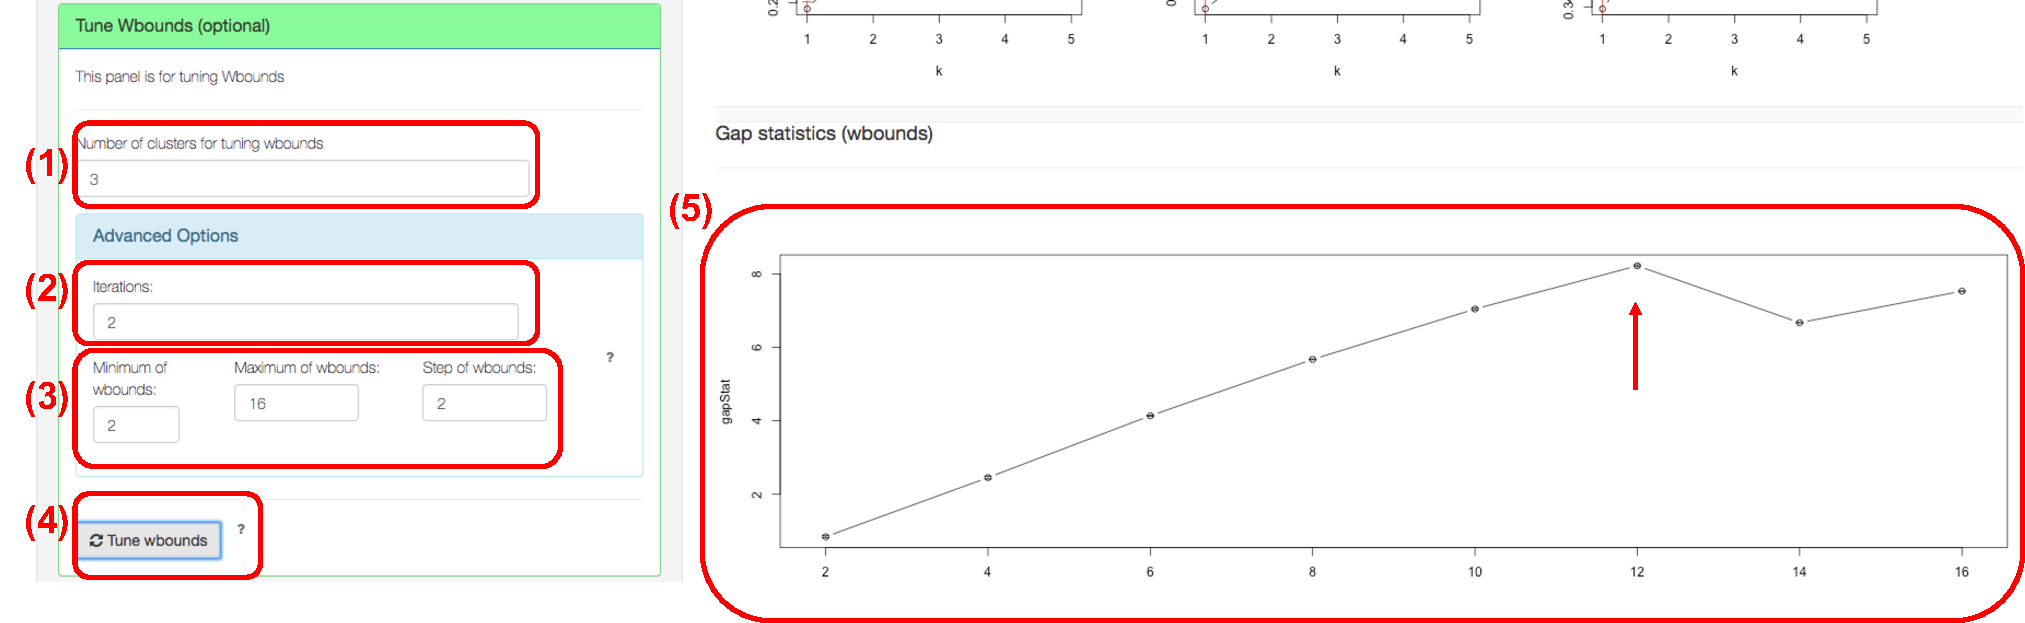
\includegraphics[scale=0.35]{./figure/metaClust/tuneW}
\caption{GUI Preprocessing page}
\label{fig:metaClusttuneW}
\end{center}
\end{figure}
Again,
gap statistics will be used for tuning Wbounds.
Users will specify number of clusters for tuning Wbounds, which could be obtained from the previous step.
Iterations is the same thing as number of bootstrap samples for gap statistics.
Users also need to specify the searching space of Wbounds by minimum of Wbounds, maximum of Wbounds and Step of Wbounds.
After all these steps are set,
user can click on ``Tune Wbounds" button.
The results will be shown in Figure~\ref{fig:metaClusttuneW}.
Wbound=12 is preferred since the corresponding gap statistics is maximized.

\subsubsection{Run Meta Sparse K-Means}
Under Run Meta Sparse K-Means panel,
user can specify number of clusters, Wbounds and run meta sparse K means, 
as in Figure~\ref{fig:mskmRes}.
\begin{figure}[H]
\begin{center}
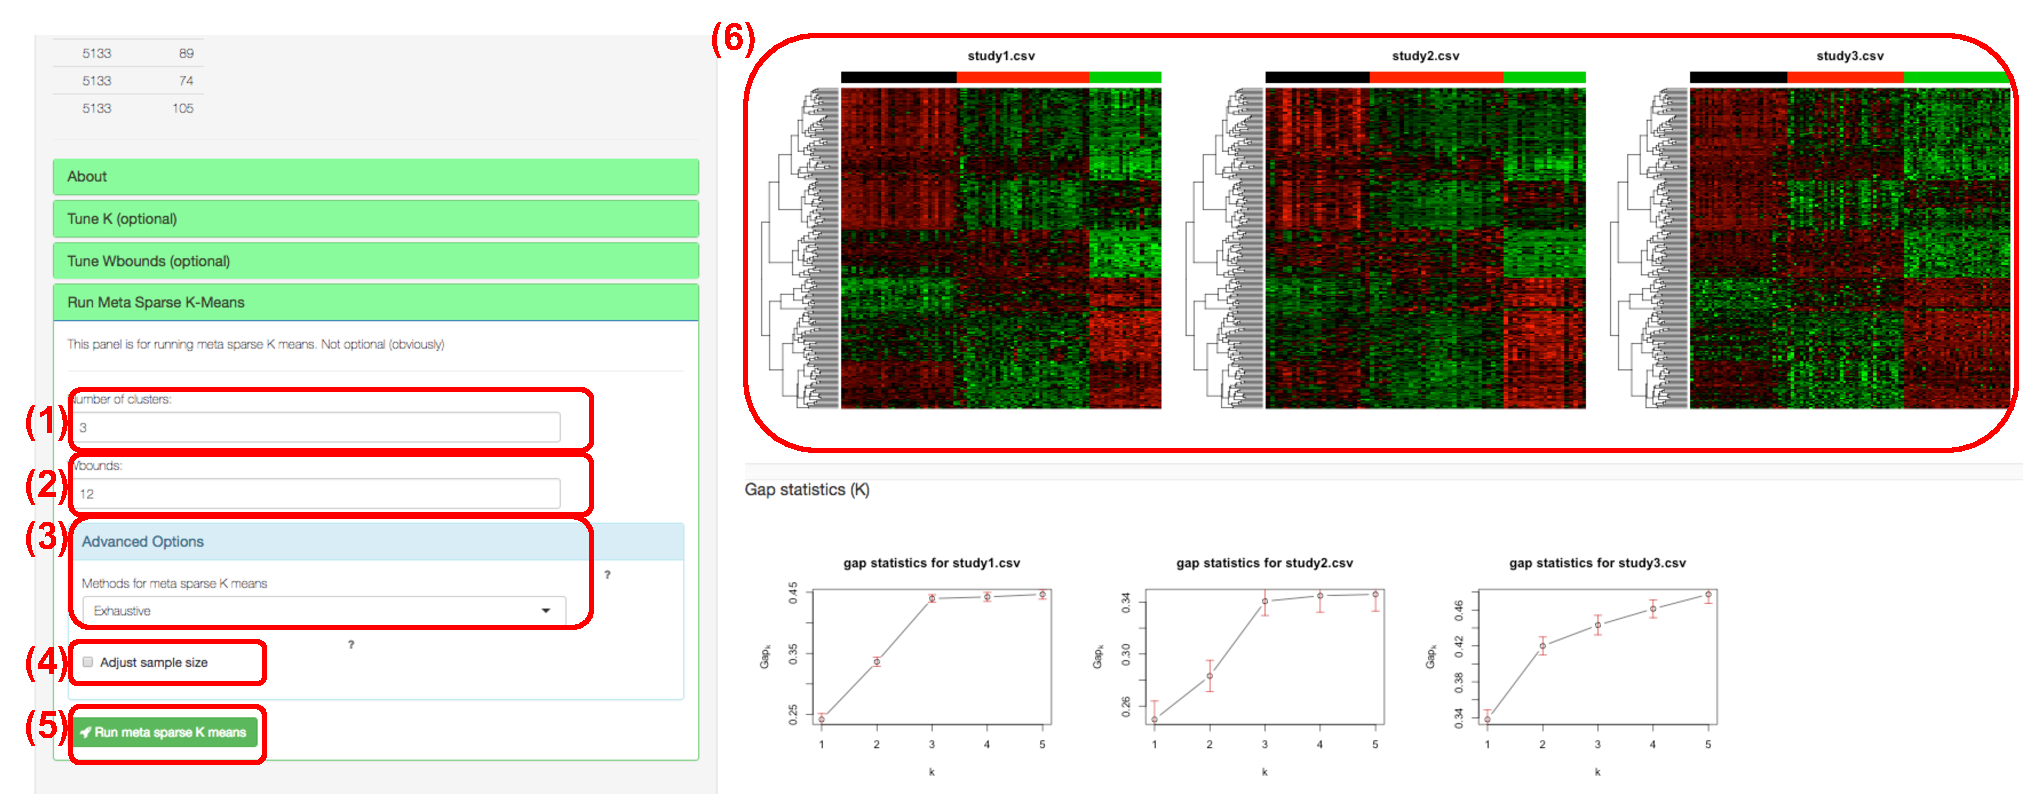
\includegraphics[scale=0.35]{./figure/metaClust/mskmRes}
\caption{GUI Preprocessing page}
\label{fig:mskmRes}
\end{center}
\end{figure}
There are three clustering matching methods: Exhaustive, linear, MCMC.
Exhaustive is suggested if the data is not large.
Linear will perform smart search and get solution much faster than Exhaustive, 
but it may yield less accuracy.
MCMC might by very time consuming.
Adjust sample size checkbox allows users to adjust sample size effect.
After number of clusters and Wbounds are specified,
users can click on Run meta sparse K means and obtain results as Figure~\ref{fig:mskmRes}.
